\section*{Neural Networks}
$F(x)=W^{L}\phi^{L-1}(W^{L-1}...(\phi^{1}(W^{1}x)...))$

$\textbf{ReLU: } \max (0,z), \; \textbf{Tanh: } \frac{\exp(z) - \exp(-z)}{\exp(z) + \exp(-z)}$ \\[-3pt]
$\textbf{Sigmoid: } \varphi(z) = \frac{1}{1 + \exp(-z)}, \varphi' = (1 - \varphi) \varphi$


\textbf{Universal Approximation Theorem}: We can approximate any arbitrary smooth target function, with 1+ layer with sufficient width.

\subsection*{Forward Propagation}

Input: $v^{(0)} = [x; 1]$ \quad Output: $f = W^{(L)} v^{(L-1)}$
Hidden: $z^{(l)} = W^{(l)} v^{(l-1)}, v^{(l)} = [\varphi(z^{(l)}); 1]$

\subsection*{Backpropagation}

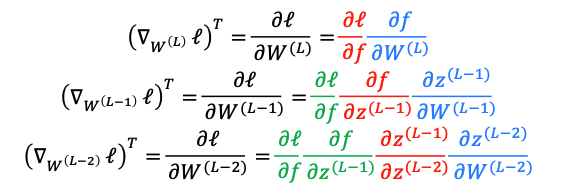
\includegraphics[width=\columnwidth]{assets/backpropagation.png} \\[-15pt]



Only compute {\color{red} \textbf{the gradient}}. Rand. init. weights by distr. assumption for $\varphi$. ( $2 / n_{in}$ for ReLu and $1/n_{in}$ or $ 2/ (n_{in} + n_{out})$ for Tanh)

\subsection*{Overfitting}
\textbf{Regularization}; \textbf{Early Stopping}; \textbf{Dropout}: 
ignore hidden units with prob. $1-p$, after training use all units 
and scale weights by $p$; 
\textbf{Batch Normalization}: normalize the input data 
for each mini-batch, rescale and shift;

\subsection*{CNN \quad \color{black}$\varphi(W * v^{(l)})$}

The out. dim. of applying $k$ $f \times f \times d$ filters (\(d\) = \# channels) to 
$n \times m$ image with padding $p$ and stride $s$ is: 
$\left(\frac{n+2p-f}{s}+1\right) \times \left(\frac{m+2p-f}{s}+1\right)$ with \(k\) channels.
If \(t\times t\) pooling is applied, both dimensions are divided by \(t\), nr. channels stays.
\textbf{Don't forget bias}: 1 per filter + \#outputs for any fully connected layer.

\subsection*{Learning with momentum}
$a \leftarrow m \cdot a + \eta_t \nabla_W l(W;y,x)$; $W \leftarrow W - a$